% template:
% Copyright 2020 by Junwei Wang <i.junwei.wang@gmail.com>
%
% This file may be distributed and/or modified under the
% conditions of the LaTeX Project Public License, either version 1.3c
% of this license or (at your option) any later version.
% The latest version of this license is in
%   http://www.latex-project.org/lppl.txt

% presentation:
% joelfaubert@gmail.com
% 3/19/2021

\documentclass[compress]{beamer}

\usepackage[english]{babel}
\usepackage{metalogo}
\usepackage{listings}
\usepackage{fontspec}
\usepackage{tikz}
\usepackage{hyperref}
\usepackage[utf8]{inputenc}

\usetheme{Nord}
% \usetheme[style=light]{Nord}

\setmainfont{Yanone Kaffeesatz}
\setsansfont{Andika New Basic}
\setmonofont{DejaVu Sans Mono}

\newcommand{\blue}[1]{\textcolor{NordBlue}{#1}}
\newcommand{\bblue}[1]{\textcolor{NordBrightBlue}{#1}}

\newcommand{\red}[1]{\textcolor{NordRed}{#1}}
\newcommand{\yellow}[1]{\textcolor{NordYellow}{#1}}
\newcommand{\magenta}[1]{\textcolor{NordMagenta}{#1}}

\newcommand{\cyan}[1]{\textcolor{NordCyan}{#1}}
\newcommand{\bcyan}[1]{\textcolor{NordBrightCyan}{#1}}

\newcommand{\white}[1]{\textcolor{NordWhite}{#1}}
\newcommand{\bwhite}[1]{\textcolor{NordBrighterWhite}{#1}}
\newcommand{\Bwhite}[1]{\textcolor{NordBrightestWhite}{#1}}


%\AtBeginSection[]
%{
%  \begin{frame}[c,noframenumbering,plain]
%    \tableofcontents[sectionstyle=show/hide,subsectionstyle=show/show/hide]
%  \end{frame}
%}

%AtBeginSubsection[]
%{
%  \begin{frame}[c,noframenumbering,plain]
%    \tableofcontents[sectionstyle=show/hide,subsectionstyle=show/shaded/hide]
%  \end{frame}
%}

\title{Combinatorial Games}
\subtitle{and fun with Unicode}
\author{Jo\"el Faubert}
%\institution{Snowed In Studios Mahomies}
\date{\today}


% document start

\begin{document}

\begin{frame}[plain,noframenumbering]

  \maketitle

  \vspace{10em}

Beamer Theme \bcyan{Nord} by

\blue{Junwei Wang} of {\it  CryptoExperts }
\end{frame}

\begin{frame}
    \tableofcontents
\end{frame}

\section{Intro}

\begin{frame}[fragile]{Combinatorial games}

\blue{Combinatorial games} are (sequential, two-player) perfect information games.

\bigskip

\blue{Combinatorics}: counting stuff, combinations, permutations.

\bigskip

\cyan{Construction}, \blue{existence} and \bcyan{optimization} of structures.

\bigskip

\begin{figure}
    \centering
\begin{tikzpicture}[sibling distance=2.5em, level distance=2.5em,
  every node/.style = {shape=circle, draw, align=center, color=white}]
  \node {a}
    child { node {b} }
      child { node {c}
        child { node {d} }
        child { node {e} } };
\end{tikzpicture}
\end{figure}
\end{frame}

\subsection{Table, Nim}
\begin{frame}{Everything's on the table}
    \textbf{Rules:}
    \begin{description}
        \item \red{Two players} take turns
        \item Place \yellow{1-10} items on the table
        \item Player to hit \bcyan{100} wins
    \end{description}
\end{frame}

\begin{frame}[fragile]{Nim}
Take as many as you like from a single pile.
\smallskip
\begin{center}
{\Huge
\blue{\fontspec{Symbola} \symbol{"26C0}}

\smallskip
\red{\fontspec{Symbola} \symbol{"26C2} \symbol{"26C2}}

\smallskip
\blue{\fontspec{Symbola} \symbol{"26C0} \symbol{"26C0} \symbol{"26C0}}

%\smallskip
%\red{\fontspec{Symbola} \symbol{"26C2} \symbol{"26C2} \symbol{"26C2} \symbol{"26C2}}
}

\end{center}

\medskip
\begin{itemize}
    \item \bcyan{normal}: last to pick up wins
    \item \bcyan{mis\`ere}: last to pick up loses
\end{itemize}

\end{frame}

\begin{frame}{Nim solution}

In normal play, the winning strategy is to finish every move with a \cyan{nim-sum} of 0.

\bigskip

\begin{table}
\centering
\begin{tabular}{c | c}
    1 & 001 \\
    2 & 010 \\
    3 & 011 \\
%    4 & 100 \\
\hline
    0 & 000
\end{tabular}

\caption{Binary digital sum of previous game}

\end{table}
\medskip
See \href{https://en.wikipedia.org/wiki/Nim}{\yellow{Wikipedia entry on Nim}} for full details.

Use nim-sum calculator or table of winning positions to defeat children.

Change size/number of heaps to keep them bewildered.

\end{frame}

\begin{frame}{Game Theory}

\begin{itemize}
    \item \cyan{Analyzing}, \blue{generating}, and \magenta{optimizing} \blue{game objects}
    \item Levels, strategies, likelihoods, and outcomes.
\end{itemize}

\bigskip

\begin{itemize}
        \item \blue{Tic tac toe}  $(9 - r)$ \red{\it possible moves} left
        \item \blue{Card} games have \href{https://en.wikipedia.org/wiki/Standard\_52-card\_deck\#Combinations}{\red{hands}}
    \item \blue{Labyrinths} have \red{paths}
\end{itemize}

\medskip
\begin{center}
\textcolor{black}{\Huge \fontspec{Symbola} \symbol{"1F0A4} \symbol{"1F0A1} \symbol{"1F0A2} \symbol{"1F0A3} \symbol{"1F0BF}}
\end{center}
\[ { 52 \choose 5} \qquad \text{Possible 5 card draws}\]
\medskip
\[G = (V,E) \qquad \min_{P\subset V \land \{ P \, \text{joins a to b} \} } |P|\]

\end{frame}


\begin{frame}{Easy games}

\bblue{Tic Tac Toe} 2nd player can force draw
\begin{figure}
    \centering
    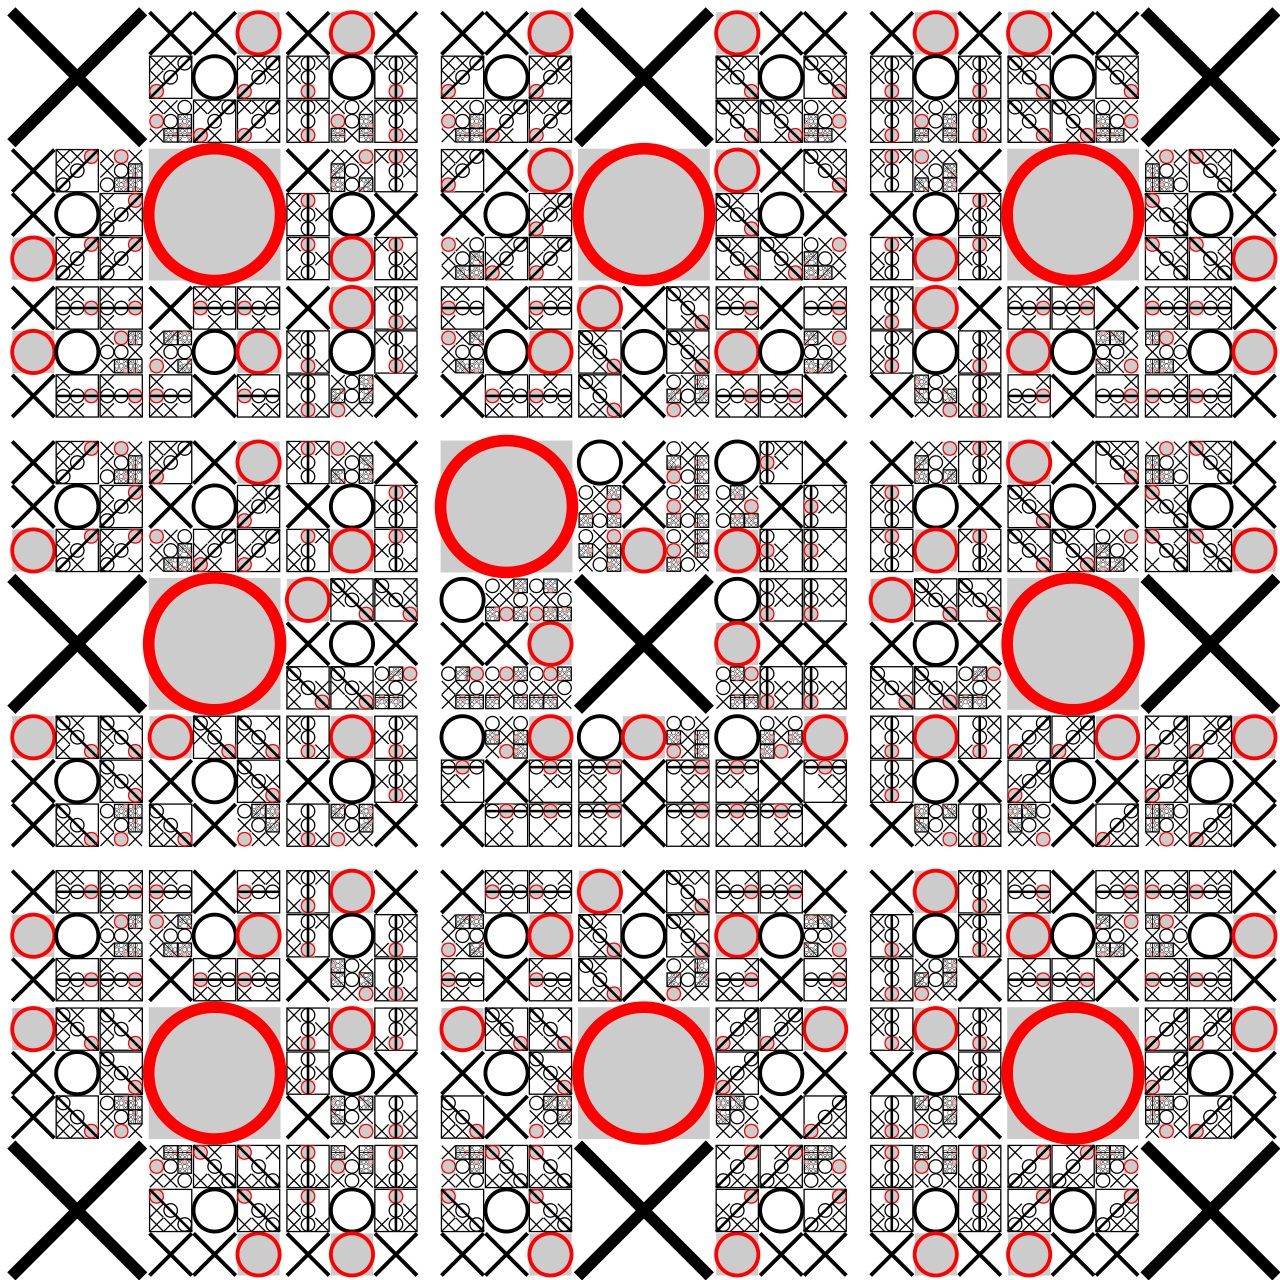
\includegraphics[scale = 0.16]{img/tic_tac_toe.jpg}
    \caption{Optimal tree for O: \href{https://en.wikipedia.org/wiki/Tic-tac-toe\#/media/File:Tictactoe-O.svg}{``A Fractal Guide to Tic Tac Toe", Ian Stewart}}
    \label{fig:tic_tac_toe}
\end{figure}
\end{frame}

\begin{frame}{Easy (?) games}

{\Huge \red{\fontspec{Symbola} \symbol{"26C2} \symbol{"26C2} \symbol{"26C2} \symbol{"26C2} \symbol{"26C2} \symbol{"26C2}}  }

\bigskip

\bblue{Nim (with 6 pieces)} 2nd player wins; algorithm for multiple heaps

\bigskip

\bblue{War} is finite (sketchy proof I dunno).
\smallskip
\end{frame}

\begin{frame}{Connect Four}

1st player has a winning strategy
\medskip
\begin{figure}
    \centering
    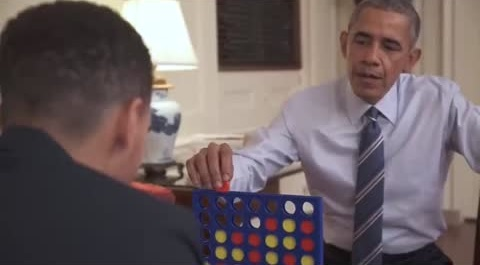
\includegraphics[width=0.8\textwidth]{img/obama_connect_four.jpg}
    \caption{Did Obama use hacks?}
    \label{fig:obama_connect_four}
\end{figure}
\end{frame}

\begin{frame}{Difficult (?) games}

\begin{description}
\item \bblue{Chess}
\begin{itemize}
    \item First automaton \yellow{The Turk} was a hoax (!)
\end{itemize}
\item \bblue{Go}
\begin{itemize}
    \item reinforcement learning AI quite good
\end{itemize}
\end{description}
\bigskip
\begin{center}
{\Large \fontspec{Symbola} \symbol{"1F4BB} > \symbol{"1F9E0} }
\end{center}
\end{frame}

\section{Categorizing Games}

\begin{frame}[fragile]
\frametitle{How much is up to chance?}

Is the game \red{probabilistic} or \blue{deterministic}?
\medskip
\begin{itemize}
\item \magenta{Pure luck}; playing against against entropy
\begin{itemize}
    \item lottery
    \item roulette
    \item dice
\end{itemize}

\item \cyan{Mix} of chance and strategy; other players
\begin{itemize}
    \item poker
    \item monopoly
    \item dota
\end{itemize}

\item \blue{Deterministic}; no luck at all
\begin{itemize}
    \item Tic tac toe
    \item Connect Four
    \item Chess
    \item Conway's Game of Life
\end{itemize}
\end{itemize}

\end{frame}

\begin{frame}{Player Information}
\yellow{Perfect information}
\begin{itemize}
    \item Tic tac toe
    \item Chess
    \item Pac-man
\end{itemize}
\bigskip
\magenta{Imperfect information}
\begin{itemize}
    \item Poker
    \item Battleships
    \item Liar's dice
\end{itemize}
\end{frame}

\begin{frame}{Sequential or Simultaneous}
\begin{itemize}
\item \yellow{Sequential}
\begin{itemize}
    \item Chess, tic tac toe, checkers, monopoly
    \item every player gets a turn, constituting a round
\end{itemize}

\item \red{Simultaneous}
\begin{itemize}
    \item Bingo
    \item War
    \item 6 Nimmt
\end{itemize}

\item \blue{Real-time}
\begin{itemize}
    \item Dota 2
    \item Hungry-hungry hippos
    \item Pong
\end{itemize}
\end{itemize}
\bigskip
{\tiny some of these last ones don't really fit; dexterity games; the challenge is in performing action}
\end{frame}

\begin{frame}{Outcomes}

\begin{itemize}
    \item \magenta{Determined}
    \begin{itemize}
        \item Win
        \item (or Lose)
    \end{itemize}
    \item \magenta{Undetermined}
    \begin{itemize}
        \item Possibility of draw
        \item Infinite play
        \item Loopy: possible to return to previous state
    \end{itemize}
\end{itemize}
\end{frame}
\begin{frame}{Strategies and sequences}

A \bcyan{players} makes a choice, a \magenta{play} or a \red{move}. May allow pass/do nothing (passive).

\medskip
Some games can be modeled as \cyan{digraphs} or \blue{state machines}: move from one valid state to the next;
strategies then are similar to outputs from Mealy or Moore machines

\medskip

\end{frame}

\begin{frame}{Game graphs of Nim}
\begin{figure}
    \centering
    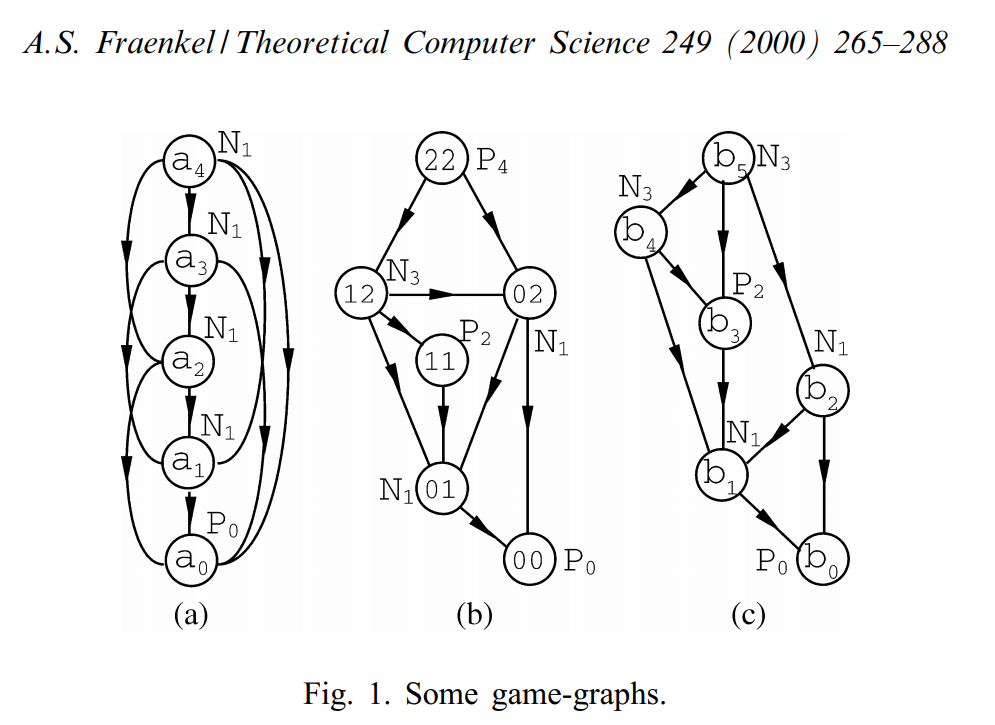
\includegraphics[width=0.75\framewidth]{img/game graphs.PNG}
    \caption{Aviezri S. Fraenkel, {\it Recent results and questions in combinatorial game complexities }}
    \label{fig:game_graphs}
\end{figure}
\end{frame}

\begin{frame}{Progressively finite}

\begin{itemize}
    \item if game digraph has \blue{no cycles}
    \item (cannot return to previous positions)
    \item the game \blue{ends} in \blue{finite} turns.
\end{itemize}

\end{frame}

\begin{frame}{Kernel of a game}
    Let $D$ be the game graph of a progressively finite game and $K \subset V(D)$. The set $K$ is called the \red{Kernel} of $D$ if it satisfies the following three
properties:

\bigskip
\begin{enumerate}
\item  all the winning vertices are in $K$
\item there is no edge from any vertex in $K$ to any (other) vertex in $K$
\item from every vertex not in $K$, there is an edge to some vertex in $K$.
\end{enumerate}
\bigskip
Kernel of the Table game:

\[ K = \{100, 89, 78, 67, 56, 45, 34, 23, 12, 1 \} \]
\end{frame}




\begin{frame}[fragile]{Portable Game Notation}

\begin{center}
\yellow{ \fontspec{Symbola} \symbol{"2654} }
\end{center}

{\tiny
\begin{lstlisting}
[Event "F/S Return Match"]
[Site "Belgrade, Serbia JUG"]
[Date "1992.11.04"]
[Round "29"]
[White "Fischer, Robert J."]
[Black "Spassky, Boris V."]
[Result "1/2-1/2"]
\end{lstlisting} }
\begin{lstlisting}
1. e4 e5 2. Nf3 Nc6 3. Bb5 a6
{This opening is called the Ruy Lopez.}
4. Ba4 Nf6 5. O-O Be7 ...
\end{lstlisting}

\bigskip
\red{ \fontspec{Symbola} \symbol{"2655} }A tournament match in \cyan{\href{https://en.wikipedia.org/wiki/Portable_Game_Notation}{Portable Game Notation}}
\end{frame}

\begin{frame}{Winner/Gagnant}

A \bcyan{strategy} can be described by a sequence of moves. A \cyan{winning} strategy is a way for one player to win \bcyan{no matter what the opponent may do}.

\medskip

\[\exists k \, : \, \exists x_1 \forall y_1 \exists x_2 \forall y_2 \dots \forall y_{k-1} \exists x_k \]

such that $x_k$ is a win for player $x$.
\end{frame}


\begin{frame}{Finding the best move}


Searching \blue{decision trees}

\bigskip

\[{\underline {v_{i}}}=\max _{a_{i}}\min _{a_{-i}}{v_{i}(a_{i},a_{-i})}\]

\smallskip

\href{https://en.wikipedia.org/wiki/Minimax}{Minimax algorithm}


\end{frame}

\begin{frame}{Uh oh factorial}
\red{Problem}: Counting all possible choices explodes.

\medskip

\red{Factorial} is bad; solving for many games is known to \cyan{NP-Complete} or \bcyan{EXPtime-Complete} (chess, go).

\medskip

Algorithms compensate by trying to explore decision trees intelligently, pruning bad moves.
\end{frame}


\section{Graph games}
\subsection{Connectivity games}
\begin{frame}{Shannon switching game}

Distinguished vertices $a$ and $b$.

\medskip

Player \blue{short} can reinforce edges.

\medskip

Player \red{cut} can remove (non-reinforced) edges.

\begin{figure}
    \centering
    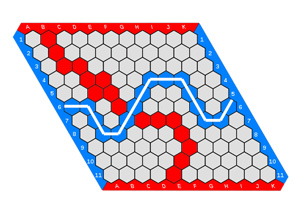
\includegraphics[scale=0.6]{img/hex_board.jpg}
    \caption{Game of \href{https://en.wikipedia.org/wiki/Hex\_(board\_game)}{Hex} (similar to shortcut)}
    \label{fig:hex}
\end{figure}
\end{frame}

\begin{frame}{Contagion and Fire}

Some nodes start on fire maybe. \red{\fontspec{Symbola} \symbol{"1F525} } \yellow{\fontspec{Symbola} \symbol{"1F525} }

\smallskip

Deploy $k$ firepeople to put out he fire.

\begin{description}
\item Firepeople
\begin{itemize}
    \item cut links of the graph,
    \item put out nodes,
    \item or protect nodes from catching
\end{itemize}

\item Fire/virus power
\begin{itemize}
    \item ability to spread
    \item eventually die out/recover
\end{itemize}
\end{description}
\end{frame}

\begin{frame}{Firefighter problem}
\begin{itemize}
    \item Invented in 1995
    \item Fire starts at node $s$, every round firefighters added to protect non-fire nodes.
    \item Goal is to \red{contain} {\fontspec{Symbola} \symbol{"1F525} }, maximizing \blue{saved} nodes
    \item NP-hard on bipartite graphs and trees with $\delta \leq 3$
    \item Even aproximation is NP-hard.

\end{itemize}

\end{frame}

\subsection{Searching games}

\begin{frame}{Searching the grid}
\newcommand*{\xMin}{0}%
\newcommand*{\xMax}{6}%
\newcommand*{\yMin}{0}%
\newcommand*{\yMax}{6}%
\begin{tikzpicture}
    \foreach \i in {\xMin,...,\xMax} {
        \draw [very thin,gray] (\i,\yMin) -- (\i,\yMax)  node [below] at (\i,\yMin) {$\i$};
    }
    \foreach \i in {\yMin,...,\yMax} {
        \draw [very thin,gray] (\xMin,\i) -- (\xMax,\i) node [left] at (\xMin,\i) {$\i$};
    }

%\draw [step=1.0,blue, very thick] (0.5,0.5) grid (5.5,4.5);
%\draw [thick, blue, step=1.0cm,xshift=-0.5cm, yshift=-0.5cm] (0.5,0.5) grid +(5.5,4.5);
%\draw [thick, blue, step=1.0cm] (1,1) grid (1, 4);
\end{tikzpicture}
\end{frame}

\begin{frame}{Searching on the line}

Place a robot on the real line at zero.

\medskip

The \red{target} is somewhere on the right ($x > 0$) or on the left ($x < 0$).

\medskip

How far do you go in one direction before deciding to turn around?

\medskip
Is there an optimal strategy? (yes)
\end{frame}

\subsection{Pursuit games}
\begin{frame}{Cops and Robbers}

Cop-number $c(G)$ of a graph: How many cops do you need to guaranteed robber will be caught?

\medskip

Aigner and Fromme showed that 3 cops have a winning strategy on a planar graph (genus 0).

\medskip

For arbitrary $g$, it has been shown that:

\[ c(G) \leq  \left\lfloor \frac{3}{2} g \right\rfloor + 3\]

\medskip

If $G$ has girth at least 5, then
\[ c(G) \geq \delta(G) \]

where $\delta(G)$ is the minimum degree of $G$.
\end{frame}


\begin{frame}{allowframebreaks}
  \begin{figure}
    \centering
    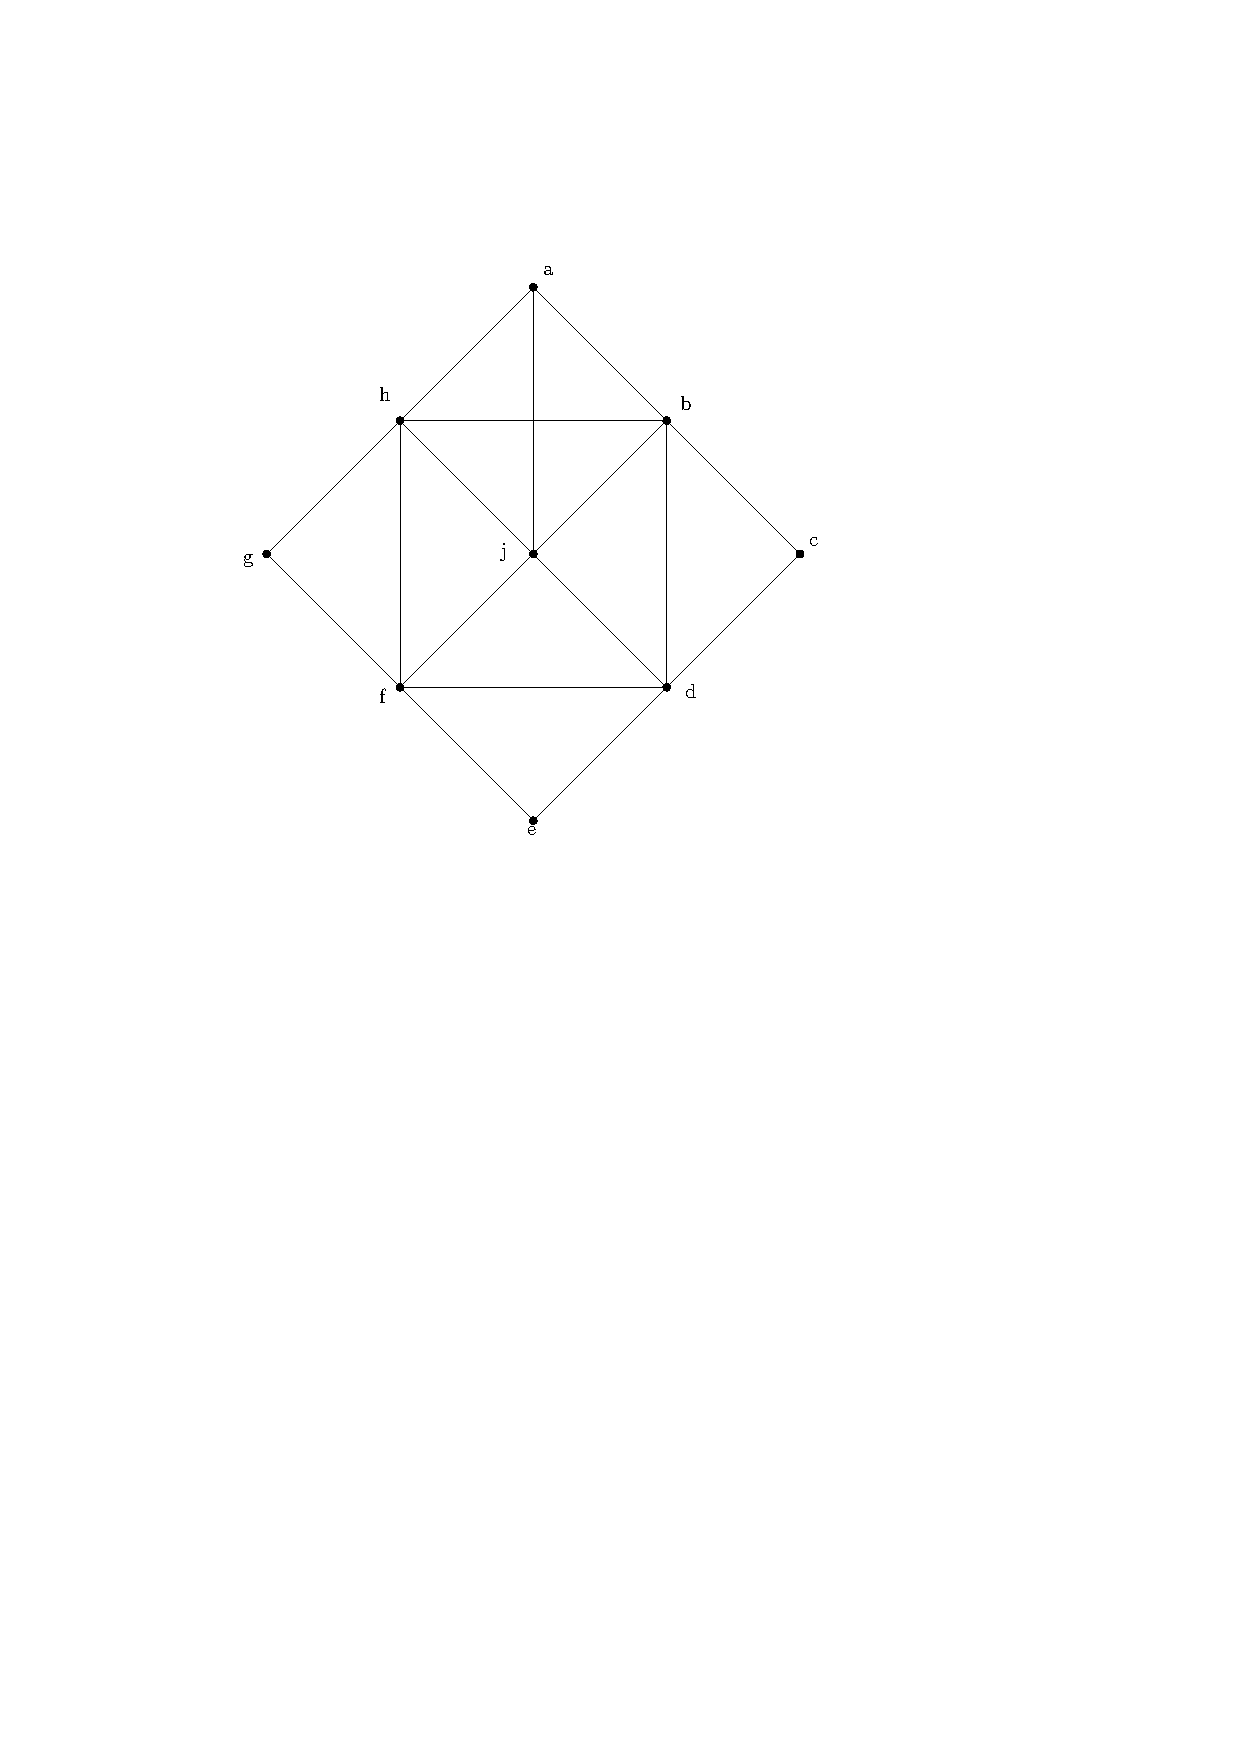
\includegraphics[width=0.8\framewidth]{img/dismantle1.pdf}
  \end{figure}
\end{frame}

\begin{frame}

  \begin{figure}
    \centering
    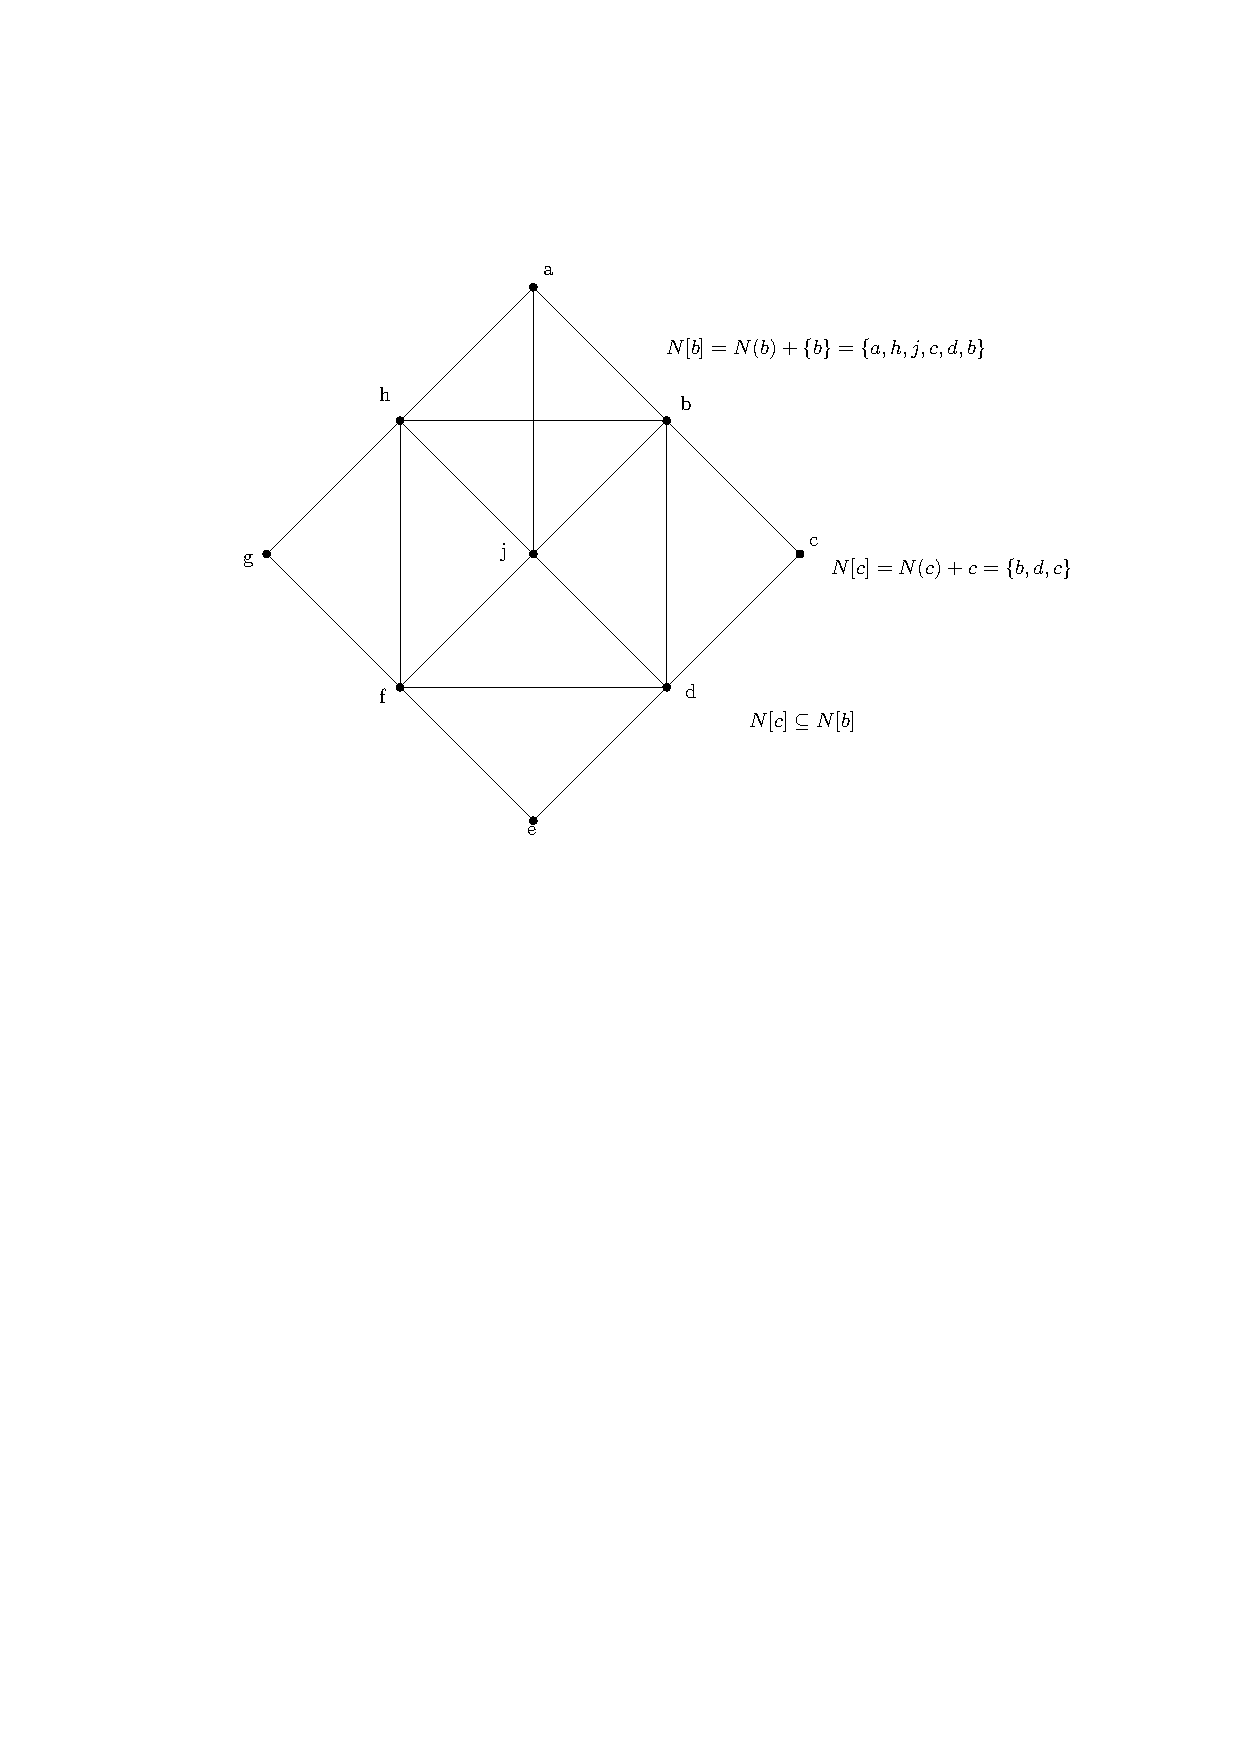
\includegraphics[width=0.8\framewidth]{img/dismantle2.pdf}
    \caption{Cop-win graph}
  \end{figure}
\end{frame}


\begin{frame}{Zombies}

What if cops were zombies instead?
\end{frame}


\begin{frame}{Gardner's Second Favourite Puzzle}

\bigskip
{\fontspec{Symbola} \huge

\textcolor{black}{🂢 	🂣 	🂤 	🂥 	🂦 	🂧 	🂨 	🂩 	🂪 	🂫 	🂬 	🂭 	🂮  🂡}
\bigskip

\textcolor{red}{🂲 	🂳 	🂴 	🂵 	🂶 	🂷 	🂸 	🂹 	🂺 	🂻 	🂼 	🂽 	🂾  🂱}
\bigskip

\textcolor{black}{🃒 	🃓 	🃔 	🃕 	🃖 	🃗 	🃘 	🃙 	🃚 	🃛 	🃜 	🃝 	🃞  🃑}

\bigskip
\textcolor{red}{🃂 	🃃 	🃄 	🃅 	🃆 	🃇 	🃈 	🃉 	🃊 	🃋 	🃌 	🃍 	🃎  🃁}
}
\end{frame}

\begin{frame}[fragile, allowframebreaks]{References}
\begin{itemize}

\item Aviezri S. Fraenkel,
Recent results and questions in combinatorial game complexities,
Theoretical Computer Science,
Volume 249, Issue 2,
2000

\item Hefetz, Dan, et al. Positional Games. Springer Basel, 2014.


\item Evgeny Lakshtanov, and Vera Roshchina. “On Finiteness in the Card Game of War.” The American Mathematical Monthly, vol. 119, no. 4, 2012, pp. 318–323. JSTOR, www.jstor.org/stable/10.4169/amer.math.monthly.119.04.318. Accessed 26 Mar. 2021.

\item Pierre Coupechoux, Marc Demange, David Ellison, Bertrand Jouve,
Firefighting on trees,
Theoretical Computer Science,
Volume 794,
2019,
Pages 69-84,

\item Anthony Bonato, Margaret-Ellen Messinger, Paweł Prałat,
Fighting constrained fires in graphs,
Theoretical Computer Science,
Volume 434,
2012,
Pages 11-22,
ISSN 0304-3975,
https://doi.org/10.1016/j.tcs.2012.01.041.
(https://www.sciencedirect.com/science/article/pii/S0304397512000989)

\item Leizhen, C., \& Weifan, W. (2009). The surviving rate of a graph for the firefighter problem. SIAM Journal on Discrete Mathematics, 23(4), 1814-13. doi:http://dx.doi.org.proxy.bib.uottawa.ca/10.1137/070700395

\item György Szabó, Gábor Fáth,
Evolutionary games on graphs,
Physics Reports,
Volume 446, Issues 4–6,
2007,
Pages 97-216,
ISSN 0370-1573,
https://doi.org/10.1016/j.physrep.2007.04.004.

\item Lehman, Alfred. "A solution of the Shannon switching game." Journal of the Society for Industrial and Applied Mathematics 12.4 (1964): 687-725.

\item Sharad S. Sane, Combinatorial Techniques, 2013.

\item Fedor V. Fomin, Pinar Heggernes, Erik Jan van Leeuwen,
The Firefighter problem on graph classes,
Theoretical Computer Science,
Volume 613,
2016,
Pages 38-50.

\item Bose, Prosenjit, Jean-Lou De Carufel, and Stephane Durocher. “Searching on a Line: A Complete Characterization of the Optimal Solution.” Theoretical computer science 569 (2015): 24–42. Web.
\end{itemize}
\end{frame}

\end{document}

%%% Local Variables:
%%% mode: latex
%%% TeX-master: t
%%% TeX-engine: xetex
%%% End:
